\section{Application objective and evidence basis}
The proposed application is supervised feedback for introductory university Python courses. Learners need diagnosis and an independently completed follow-up; teachers need control over hints, error review, and workload; departments buy and integrate the service. These are separate user, adopter, and buyer decisions. Existing assets are executable task families, trained-model baselines, program verification, and topic-scoped memory. Teacher dashboards, institutional permissions, LMS integration, correction/deletion workflows, and production monitoring remain undeveloped.

Following the business-plan guide~\cite{businesscambridge}, this chapter links use case, competition, operations, finance, and validation. Sources were checked through 7 November 2026, prioritizing original research, official statistics, and supplier documentation. Product directories inform product formats, not revenue evidence. The three evidence classes remain distinct: the data, training, and agent studies measure prototype behavior; external studies and websites describe other systems; pricing, demand, workload, conversion, and collection are commercial assumptions. No customer interview, logged-in competitor benchmark, paid teaching API trial, school purchase, or real-student pilot was conducted.

The workflow would import teacher-approved questions/tests/hint limits, require a student's own prediction or code, verify facts, supply staged feedback, route exceptions to teachers, write correctable answer evidence, and select a related follow-up. It initially supports only the declared Python subset and does not automatically grade high-stakes examinations. Original the agent study's seven complete cases out of 12 depend on tools/templates, not adopted model teaching; subsequent engineering repairs and SFT deployments do not establish institutional readiness.

\begin{figure}[htbp]\centering
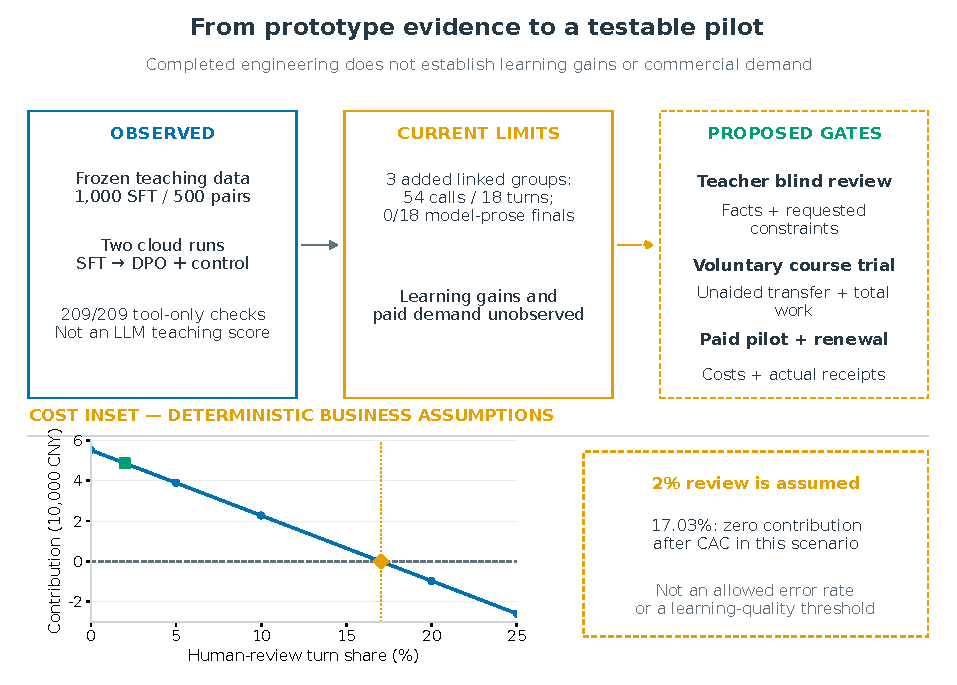
\includegraphics[width=\linewidth]{../../assets/en/evidence-to-pilot.pdf}
\caption{From research evidence to a proposed supervised pilot. Observed prototype results, external supplier claims, and business assumptions have different evidential roles. The assumed 2\% review rate and 17.03\% cost boundary are not measured quality or customer outcomes.}\label{fig:concise-business-evidence}
\end{figure}\FloatBarrier

\subsection{What external research does and does not establish}
The Ministry of Education reports 3167 higher-education institutions and 48.7257 million enrolments in 2025, across education forms~\cite{businessmoe}. Without a verified target-department list, Python enrolments, budgets, or procurement intentions, these are background rather than a validated market estimate.

Kestin et al.'s two-week, two-lesson physics crossover includes 194 of 233 enrolled students and finds benefits of an expert-designed AI tutor on immediate post-tests~\cite{businesskestin}; this system-specific result is not the project's effect. Bastani et al.'s mathematics experiment with nearly 1000 students at one Turkish high school finds approximately 17\% lower unaided exam performance for unguarded GPT Base relative to controls---a relative change, not percentage points. The guarded GPT Tutor does not demonstrate a significant positive gain on that corresponding exam outcome~\cite{businessbastani}. CodeAid's 12-week deployment in a 700-student programming course, with roughly 8000 interactions, emphasizes cognitive engagement and avoiding direct answer writing~\cite{businesscodeaid}. Together these studies motivate a pilot that separately measures assisted practice, unaided transfer, delayed retention, and teacher work; they cannot be pooled into a product ranking or a claim of demand.

\section{Competitors and differentiation hypothesis}
CodeGrade is a direct comparator for programming assignments, tests, feedback, and teacher workflow. Khanmigo is a broader tutoring and institutional-procurement comparator. Their selection reflects task relevance, not market-share rank. Table~\ref{tab:concise-business-competitors} uses archived official statements; an unverified feature is not necessarily absent.

\begin{table}[htbp]\centering\small
\caption{Officially described capabilities versus current prototype status (7 November 2026).}\label{tab:concise-business-competitors}
\begin{tabularx}{\linewidth}{@{}p{23mm}Y Y Y@{}}\toprule
Dimension & CodeGrade & Khanmigo & This project\\\midrule
Scope & Programming submissions, testing, automated grading & Cross-subject tutor, coding help, teacher/school offerings & Introductory Python research prototype\\
Teacher and evidence controls & Assignment-level hints/assistant; conversation review; code and student-visible AutoTest context & Teacher tools and institutional access; equivalent execution traces not verified here & Restricted interpreter and raw audit logs; dashboard/permissions unimplemented\\
Integration and memory & LMS integration in Advanced/institutional plans; history review, equivalent topic counters unverified & School rostering/SSO; recent-work summaries, equivalent counters unverified & Local SQLite; S02 original defect and separate repair retained; no institutional deployment\\
Procurement & Course plans and institutional quotations & Free teacher tools, personal subscription, school quotations & Proposed course service; no contract or transaction evidence\\\bottomrule
\end{tabularx}
\par\smallskip\raggedright\scriptsize Sources: CodeGrade official pricing/product/help/releases~\cite{businesscgprice,businesscgai,businesscghelp,businesscgrelease}; Khanmigo pricing/FAQs~\cite{businesskhanprice,businesskhan}. Supplier claims were not verified through same-task account trials.
\end{table}\FloatBarrier

CodeGrade lists a free plan up to 50 students/course; Starter \$24/student/course, Advanced \$39, and AI add-on \$15, with institutional quotation~\cite{businesscgprice}. The retrieved body did not explicitly establish ISO currency/tax terms, so the website's ``\$'' notation is retained without renminbi conversion. Help still calls the assistant Beta while a September 2026 release describes a paid add-on; entitlements require procurement confirmation~\cite{businesscghelp,businesscgrelease}. Khanmigo lists free teacher tools, \$4/month or \$44/year individual/family access excluding sales tax, and quoted school plans~\cite{businesskhanprice}. Individual/parent access requires adulthood, US residence and billing; teacher tools have broader geographic coverage~\cite{businesskhan,businesskhangeo}. Chinese-university contracts, data residency, and availability were not established for either supplier. Personal, course, and institutional prices are not directly comparable.

General assistants also substitute: official ChatGPT Study Mode descriptions include free-plan access, guided questions, optional memory, and error/plan limitations~\cite{businessstudymode}. Teacher visibility and test context are already public CodeGrade features. The testable differentiation is therefore lower total Chinese-course adaptation, diagnosis, and record-correction work, rather than multi-agent novelty. Teacher-authorized mappings, verified error cases, and delivery experience might accumulate, but there is no demonstrated technical moat. Existing LMS plus a general assistant is a relevant alternative.

\section{Conditional business model and unit economics}
The assumed annual departmental contract covers 300 enrolments/semester for two semesters, or 600 student--course enrolments, not necessarily 600 unique people. At CNY 120 per enrolment/semester, annual contract value is CNY 72000. Usage caps, overages, permissions, and integration must be contracted. Proposed acquisition proceeds from teacher pilot to academic approval, IT review, and budget procurement. A planning funnel of 100 screened departments, 20 qualified opportunities, 10 demonstrations, and three contracts has no observed prospect list. Three year-end contracts mean CNY 216000 annualized contracted value, not current-year receipts or recognized revenue.

At an assumed buyer-time value of CNY 90/hour, the CNY 72000 fee needs 800 net hours saved, or 80 minutes per enrolment, to pay for itself through time alone. Twenty minutes yields only CNY 18000/year. This is valuation arithmetic, not observed savings, and unreduced salaries are not cash savings.

\subsection{Cost model and stress conditions}
Assume 120 feedback turns/enrolment, with \emph{all three roles together} consuming 4500 input/900 output tokens per turn and retry multiplier $k=1.10$. The cost reference is public qwen-plus real-time non-thinking pricing in North China 2 (Beijing), input up to 128k: CNY 0.8/input-million and 2/output-million tokens, without discounts~\cite{businessprice}. This larger API model was not tested for teaching or latency and is not Chapter 2's trained 0.5B model.

For annual enrolments $N$, turns $s$, total role tokens $T$, token prices $p$, review proportion $r$, minutes $m$, and hourly outsourced cost $w$:
\begin{align}
C_{\rm API}&=Nsk\frac{T_{\rm in}p_{\rm in}+T_{\rm out}p_{\rm out}}{10^6},\\
C_{\rm review}&=Nsr\frac{m}{60}w,\\
G&=NP-C_{\rm API}-C_{\rm review}-C_{\rm setup}-C_{\rm cloud}-C_{\rm acquisition}.
\end{align}
The token totals already include three calls and must not be multiplied by three again. $P$ is price per enrolment. $G$ is contribution after delivery and incremental acquisition, before fixed company costs, not profit or fully allocated CAC. Baseline assumptions are 2\% review, three minutes/review, CNY 90/hour, 80 setup hours, CNY 1200 dedicated cloud/year, and CNY 8000 acquisition/new contract. Outsourced variable hours are not duplicated in fixed payroll. None of these is a received quotation.

\begin{figure}[htbp]\centering
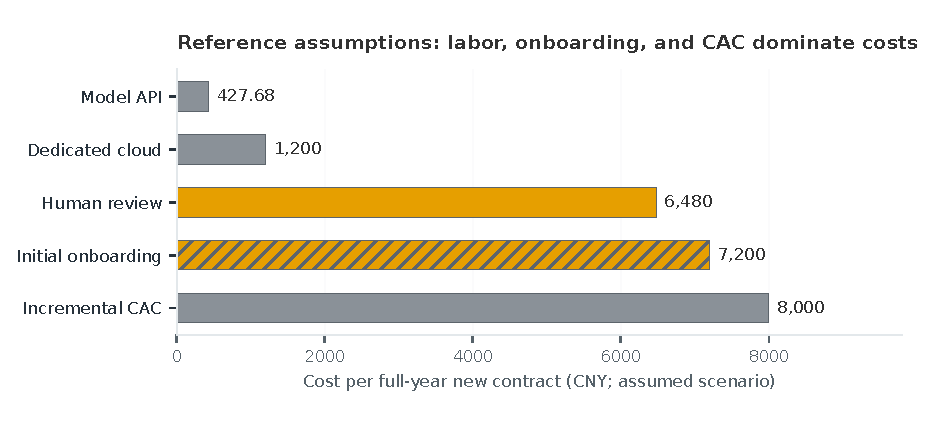
\includegraphics[width=\linewidth]{../../assets/en/business-costs.pdf}
\caption{Baseline assumed costs per full-year contract. API is an external price times assumed usage. Labor, setup, cloud, and acquisition are planning inputs; fixed company costs are separate.}\label{fig:concise-business-costs}
\end{figure}\FloatBarrier

\begin{table}[htbp]\centering\small
\caption{Baseline and joint stress assumptions. Amounts are CNY per full-year new contract; complete inputs and the efficiency scenario remain in supplementary data.}\label{tab:concise-business-finance}
\begin{tabularx}{\linewidth}{@{}Yrr@{}}\toprule
Item & Baseline & Joint stress\\\midrule
Price/enrolment; turns/enrolment &120; 120&90; 180\\
Review proportion; minutes/review &2\%; 3&5\%; 5\\
Annual revenue &72000&54000\\
Delivery cost &15307.68&54072\\
Incremental acquisition &8000&15000\\
Contribution after delivery/acquisition &48692.32&$-15072$\\\bottomrule
\end{tabularx}
\end{table}\FloatBarrier

Baseline delivery comprises CNY 427.68 API, 6480 review, 7200 setup, and 1200 cloud. Direct contribution margin before acquisition is 78.74\%. Joint stress also uses 120 setup hours and CNY 1800 cloud. Expansion cannot repair its negative contribution. Annual fixed spending assumes CNY 600000 (50000/month, including 42000 personnel). It needs 13 baseline full-year contracts, or 15 including CNY 100000 startup cost; this static calculation is not the first year with staggered starts. No scenario probabilities, lifetime value, or renewal forecast are inferred.

\begin{figure}[htbp]\centering
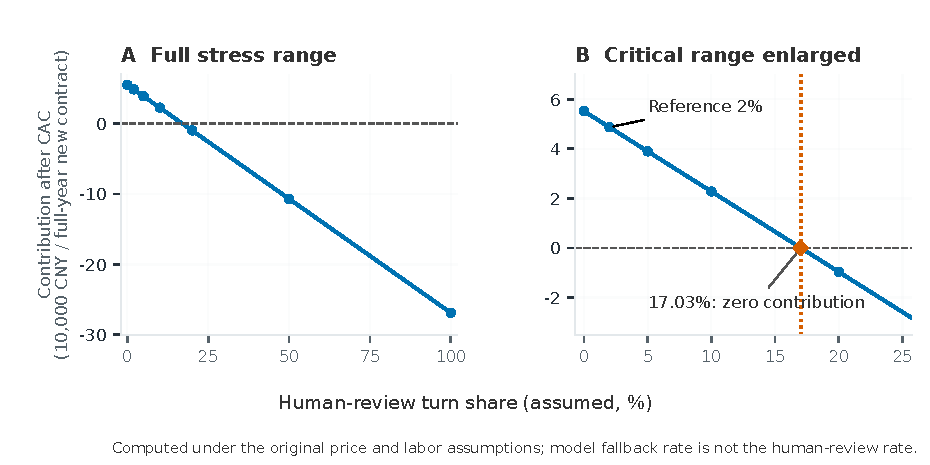
\includegraphics[width=\linewidth]{../../assets/en/business-review-stress.pdf}
\caption{Manual-review sensitivity holding other baseline assumptions fixed. The zero-contribution point near 17.03\% is commercial capacity, not an acceptable quality threshold or an observed review rate.}\label{fig:concise-business-review}
\end{figure}\FloatBarrier

At 10\%, 20\%, and 50\% review, annual contributions are CNY 22772.32, $-9627.68$, and $-106827.68$. Model non-adoption or fallback frequency cannot be converted into business review probability. If required quality costs more than the 17.03\% break-even burden, raise price, narrow scope, or stop productization; quality protection must not be lowered to meet margin.

\subsection{Cash plan and simulated funding}
A simulated CNY 1 million raise supports 12 months of engineering/pilot/procurement validation, without an asserted valuation or exit return. Annual contracts start in months 4, 7, and 10, invoice at activation, and pay three months later. Revenue is spread over service months for planning, not formal accounting. The plan includes CNY 100000 initial spending, 50000/month fixed costs, and activation-linked integration/acquisition plus usage. Actual acquisition expenditure may occur earlier than this simplified timing.

\begin{figure}[htbp]\centering
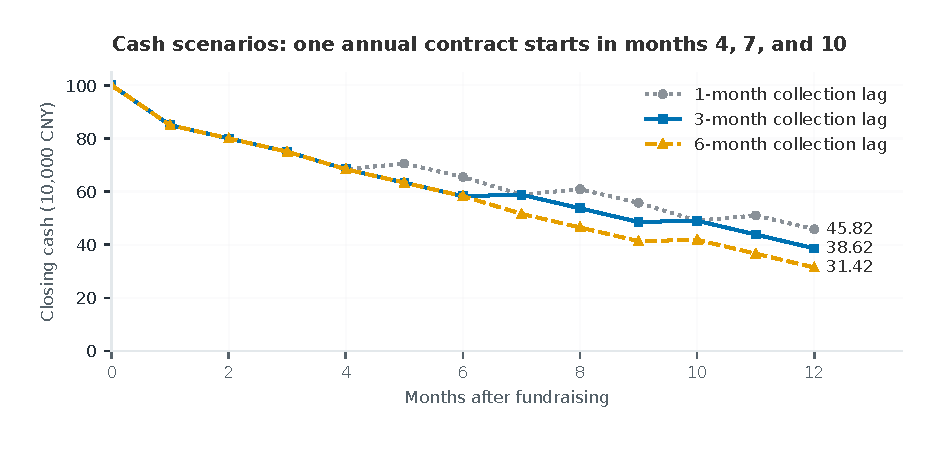
\includegraphics[width=\linewidth]{../../assets/en/business-cash.pdf}
\caption{Cash under one-, three-, and six-month collection lags, starting with assumed CNY 1 million funding. Contract starts and collections have not occurred.}\label{fig:concise-business-cash}
\end{figure}\FloatBarrier

The three-month baseline yields CNY 108000 allocated first-year revenue, 144000 receipts, and 216000 year-end annualized contracts. Approximately 757800 cash spending leaves 386200; the month-10 contract pays in year 2. Remaining cash funds future delivery and is not profit. Tax, financing, bad debt, refunds, and hardware are excluded. Local the agent study runtime does not establish production latency or cloud capacity. Pilot delay requires a revised cash plan.

\section{Validation gates and decision}
The next step is a supervised pilot conditional on further content checks, rather than automatic progression to selling. Engineering repair of known C08/S02 inputs is complete; independent teacher review, student learning evaluation, and procurement remain pending.

\begin{table}[htbp]\centering\small
\caption{Proposed evidence collection and release conditions; these are plans, not achieved outcomes.}\label{tab:concise-business-gates}
\begin{tabularx}{\linewidth}{@{}p{29mm}Y@{}}\toprule
Stage & Evidence and decision boundary\\\midrule
Content verification & New independent questions and 100 blinded teacher reviews; zero severe errors for release, with immediate pause for serious misleading feedback, unauthorized action, or memory contamination.\\
Course pilot & Two courses/about 100 voluntary learners; randomize within courses where feasible, count all preparation/review/correction/maintenance work, and test unaided transfer two weeks later with blinded grading. This sample estimates feasibility/variance, not guaranteed power.\\
Quality and workload & Proposed misleading rate $\leq2\%$, net time saving $\geq20\%$, and post-test difference versus control no worse than $-5$ points on a 100-point scale. Pre-register analysis and report intervals; an interval crossing a gate means uncertainty. Zero misleading responses in 100 independent items gives a one-sided 95\% upper bound of 2.95\%; supporting the 2\% error-rate gate requires at least 149 independent items with no misleading response. Repeated items from the same learner may not be independent.\\
Purchase and delivery & Interview 15 teachers/five procurement roles; record current workflow before demonstration, refusals, quotations, signing, invoicing, and receipts separately. Three expressions of interest are a target, not three customers.\\\bottomrule
\end{tabularx}
\end{table}\FloatBarrier

A 20\% time saving covers the assumed fee through labor value alone only if baseline work is at least 400 minutes/enrolment; this workload has not been measured. Otherwise pricing needs revision or separately evidenced benefits. Severe events are tracked separately from average error rates. A pilot needs teacher-agreed gates, contamination/withdrawal records, and a control using existing support. Team needs are engineering, curriculum evaluation, and customer delivery; no recruited team or school partnership is implied.

Future handling of learner identifiers and error histories requires a processing basis, minimized fields, retention limits, correction/deletion, commissioned-processing responsibilities, and applicable impact assessment~\cite{businesspipl}. Proposed pseudonyms, course access, and correction audits are not implemented compliance certification. Production additionally requires execution isolation, concurrency/security tests, supplier/version control, and verified procurement/data terms. Free substitutes, adaptation labor, delays, and renewals remain commercial risks. If only intensive human service is reliable, it must be priced honestly as such; negative contribution is a stopping condition.

The evidence supports bounded preparation for supervised validation, not autonomous tutoring, competitive superiority, or proven willingness to pay. Full source snapshots, 21-source ledger, three financial scenarios, 25 sensitivity combinations, monthly cash, interview/review forms, and calculation code remain under \path{business/} and \path{business/validation/}. 
